% Options for packages loaded elsewhere
\PassOptionsToPackage{unicode}{hyperref}
\PassOptionsToPackage{hyphens}{url}
%
\documentclass[
  12pt,
  a4paper,
  DIV=11,
  numbers=noendperiod]{scrreprt}

\usepackage{amsmath,amssymb}
\usepackage{setspace}
\usepackage{iftex}
\ifPDFTeX
  \usepackage[T1]{fontenc}
  \usepackage[utf8]{inputenc}
  \usepackage{textcomp} % provide euro and other symbols
\else % if luatex or xetex
  \usepackage{unicode-math}
  \defaultfontfeatures{Scale=MatchLowercase}
  \defaultfontfeatures[\rmfamily]{Ligatures=TeX,Scale=1}
\fi
\usepackage{lmodern}
\ifPDFTeX\else  
    % xetex/luatex font selection
\fi
% Use upquote if available, for straight quotes in verbatim environments
\IfFileExists{upquote.sty}{\usepackage{upquote}}{}
\IfFileExists{microtype.sty}{% use microtype if available
  \usepackage[]{microtype}
  \UseMicrotypeSet[protrusion]{basicmath} % disable protrusion for tt fonts
}{}
\usepackage{xcolor}
\setlength{\emergencystretch}{3em} % prevent overfull lines
\setcounter{secnumdepth}{5}
% Make \paragraph and \subparagraph free-standing
\ifx\paragraph\undefined\else
  \let\oldparagraph\paragraph
  \renewcommand{\paragraph}[1]{\oldparagraph{#1}\mbox{}}
\fi
\ifx\subparagraph\undefined\else
  \let\oldsubparagraph\subparagraph
  \renewcommand{\subparagraph}[1]{\oldsubparagraph{#1}\mbox{}}
\fi


\providecommand{\tightlist}{%
  \setlength{\itemsep}{0pt}\setlength{\parskip}{0pt}}\usepackage{longtable,booktabs,array}
\usepackage{calc} % for calculating minipage widths
% Correct order of tables after \paragraph or \subparagraph
\usepackage{etoolbox}
\makeatletter
\patchcmd\longtable{\par}{\if@noskipsec\mbox{}\fi\par}{}{}
\makeatother
% Allow footnotes in longtable head/foot
\IfFileExists{footnotehyper.sty}{\usepackage{footnotehyper}}{\usepackage{footnote}}
\makesavenoteenv{longtable}
\usepackage{graphicx}
\makeatletter
\def\maxwidth{\ifdim\Gin@nat@width>\linewidth\linewidth\else\Gin@nat@width\fi}
\def\maxheight{\ifdim\Gin@nat@height>\textheight\textheight\else\Gin@nat@height\fi}
\makeatother
% Scale images if necessary, so that they will not overflow the page
% margins by default, and it is still possible to overwrite the defaults
% using explicit options in \includegraphics[width, height, ...]{}
\setkeys{Gin}{width=\maxwidth,height=\maxheight,keepaspectratio}
% Set default figure placement to htbp
\makeatletter
\def\fps@figure{htbp}
\makeatother

\usepackage{indentfirst}
\usepackage{float}
\floatplacement{figure}{H}
\IfFileExists{plex-otf.sty}{
  %% Full TeXlive
  \usepackage[
    % math,
    RM={Scale=0.94},SS={Scale=0.94},SScon={Scale=0.94},TT={Scale=MatchLowercase,FakeStretch=0.9},
    DefaultFeatures={Ligatures=Common}
  ]{plex-otf}
  % \usepackage[Scale=MatchUppercase]{juliamono}
}{
  %% TinyTeX
  \usepackage{libertine}
}
\KOMAoption{captions}{tableheading}
\makeatletter
\@ifpackageloaded{caption}{}{\usepackage{caption}}
\AtBeginDocument{%
\ifdefined\contentsname
  \renewcommand*\contentsname{Содержание}
\else
  \newcommand\contentsname{Содержание}
\fi
\ifdefined\listfigurename
  \renewcommand*\listfigurename{Список иллюстраций}
\else
  \newcommand\listfigurename{Список иллюстраций}
\fi
\ifdefined\listtablename
  \renewcommand*\listtablename{Список таблиц}
\else
  \newcommand\listtablename{Список таблиц}
\fi
\ifdefined\figurename
  \renewcommand*\figurename{Рисунок}
\else
  \newcommand\figurename{Рисунок}
\fi
\ifdefined\tablename
  \renewcommand*\tablename{Таблица}
\else
  \newcommand\tablename{Таблица}
\fi
}
\@ifpackageloaded{float}{}{\usepackage{float}}
\floatstyle{ruled}
\@ifundefined{c@chapter}{\newfloat{codelisting}{h}{lop}}{\newfloat{codelisting}{h}{lop}[chapter]}
\floatname{codelisting}{Список}
\newcommand*\listoflistings{\listof{codelisting}{Листинги}}
\makeatother
\makeatletter
\makeatother
\makeatletter
\@ifpackageloaded{caption}{}{\usepackage{caption}}
\@ifpackageloaded{subcaption}{}{\usepackage{subcaption}}
\makeatother
\ifLuaTeX
\usepackage[bidi=basic]{babel}
\else
\usepackage[bidi=default]{babel}
\fi
\babelprovide[main,import]{russian}
\babelprovide[import]{english}
% get rid of language-specific shorthands (see #6817):
\let\LanguageShortHands\languageshorthands
\def\languageshorthands#1{}
\ifLuaTeX
  \usepackage{selnolig}  % disable illegal ligatures
\fi
\usepackage[style=gost-numeric,backend=biber,langhook=extras,autolang=other*]{biblatex}
\addbibresource{bib/cite.bib}
\usepackage{csquotes}
\usepackage{bookmark}

\IfFileExists{xurl.sty}{\usepackage{xurl}}{} % add URL line breaks if available
\urlstyle{same} % disable monospaced font for URLs
\hypersetup{
  pdftitle={Отчёта по лабораторной работе 8},
  pdfauthor={Нджову Нелиа},
  pdflang={ru-RU},
  hidelinks,
  pdfcreator={LaTeX via pandoc}}

\title{Отчёта по лабораторной работе 8}
\usepackage{etoolbox}
\makeatletter
\providecommand{\subtitle}[1]{% add subtitle to \maketitle
  \apptocmd{\@title}{\par {\large #1 \par}}{}{}
}
\makeatother
\subtitle{Математическое моделирование}
\author{Нджову Нелиа}
\date{}

\begin{document}
\maketitle

\renewcommand*\contentsname{Содержание}
{
\setcounter{tocdepth}{1}
\tableofcontents
}
\listoffigures
\listoftables
\setstretch{1.5}
\chapter{Цель
работы}\label{ux446ux435ux43bux44c-ux440ux430ux431ux43eux442ux44b}

Целью данной лабораторной работы является построение математической
модели конкуренции двух фирм.

\chapter{Задание}\label{ux437ux430ux434ux430ux43dux438ux435}

\textbf{Вариант 64}

\textbf{Случай 1.} Рассмотрим две фирмы, производящие взаимозаменяемые
товары одинакового качества и находящиеся в одной рыночной нише.
Считаем, что в рамках нашей модели конкурентная борьба ведётся только
рыночными методами. То есть, конкуренты могут влиять на противника путем
изменения параметров своего производства: себестоимость, время цикла, но
не могут прямо вмешиваться в ситуацию на рынке («назначать» цену или
влиять на потребителей каким-либо иным способом.) Будем считать, что
постоянные издержки пренебрежимо малы, и в модели учитывать не будем. В
этом случае динамика изменения объемов продаж фирмы 1 и фирмы 2
описывается следующей системой уравнений:

\[
\frac{dM_1}{d\theta} = M_1 - \frac{b}{c_1}M_1M_2 - \frac{a_1}{c_1}M1^2
\] \[
\frac{dM_2}{d\theta} = \frac{c_2}{c_1}M_2 - \frac{b}{c_1}M_1M_2 - \frac{a_2}{c_1}M_2^2
\]

где: \(a_1 = \frac{p_{cr}}{\tau_1^2p̃_1^2Nq}\),
\(a_2 = \frac{p_{cr}}{\tau_2^2p̃_2^2Nq}\),
\(b = \frac{p_{cr}}{\tau_1^2p̃_1^2\tau_2^2p̃_2^2Nq}\),
\(c_1 = \frac{p_{cr} - p̃_1}{\tau_1p̃_1}\),
\(c_2 = \frac{p_{cr} - p̃_2}{\tau_2p̃_2}\)

Также введена нормировка t = c1\(\theta\)

\textbf{Случай 2}. Рассмотрим модель, когда, помимо экономического
фактора влияния (изменение себестоимости, производственного цикла,
использование кредита и т.п.), используются еще и
социально-психологические факторы -- формирование общественного
предпочтения одного товара другому, не зависимо от их качества и цены. В
этом случае взаимодействие двух фирм будет зависеть друг от друга,
соответственно коэффициент перед \(M_1*M_2\) будет отличаться. Пусть в
рамках рассматриваемой модели динамика изменения объемов продаж фирмы 1
и фирмы 2 описывается следующей системой уравнений:

\[
\frac{dM_1}{d\theta} = M_1 - \left(\frac{b}{c_1} + 0.00064\right)M_1M_2 - \frac{a_1}{c_1}M1^2
\] \[
\frac{dM_2}{d\theta} = \frac{c_2}{c_1}M_2 - \frac{b}{c_1}M_1M_2 - \frac{a_2}{c_1}M_2^2
\]

Для обоих случаев рассмотрим задачу со следующими начальными условиями и
параметрами:

\(M_0^1 = 6.1\), \(M_0^2 = 4.5\), \(p_{cr} = 31\), \(N = 30\),
\(q = 1\), \(\tau_1 = 15\), \(\tau_2 = 17\), \(p̃_1 = 9.7\),
\(p̃_2 = 8.4\)

\textbf{\emph{Замечание:}} Значения \(p_{cr}, p_{1,2}, N\) указаны в
тысячах единиц, а значения \(M_{1,2}\) указаны в млн. единиц.

\textbf{\emph{Обозначения:}}

N -- число потребителей производимого продукта.

\(\tau\) -- длительность производственного цикла

p -- рыночная цена товара

p̃ -- себестоимость продукта, то есть переменные издержки на производство
единицы продукции.

q -- максимальная потребность одного человека в продукте в единицу
времени1

\(\theta = \frac{t}{c_1}\) - безразмерное время

\begin{enumerate}
\def\labelenumi{\arabic{enumi}.}
\item
  Постройте графики изменения оборотных средств фирмы 1 и фирмы 2 без
  учета постоянных издержек и с веденной нормировкой для случая 1.
\item
  Постройте графики изменения оборотных средств фирмы 1 и фирмы 2 без
  учета постоянных издержек и с веденной нормировкой для случая 2.
\end{enumerate}

\chapter{Теоретическое
введение}\label{ux442ux435ux43eux440ux435ux442ux438ux447ux435ux441ux43aux43eux435-ux432ux432ux435ux434ux435ux43dux438ux435}

Математическому моделированию процессов конкуренции и сотрудничества
двух фирм на различных рынках посвящено довольно много научных работ, в
основном использующих аппарат теории игр и статистических решений. В
качестве примера можно привести работы таких исследователей, как Курно,
Стакельберг, Бертран, Нэш, Парето {[}1{]}.

Следует отметить, что динамические дифференциальные модели уже давно и
успешно используются для математического моделирования самых
разнообразных по своей природе процессов. Достаточно упомянуть широко
использующуюся в экологии модель «хищник-жертва» Вольтерра,
математическую теорию развития эпидемий, модели боевых действий Задача
решалась в следующей постановке {[}2{]}.

На рынке однородного товара присутствуют две основные фирмы, разделяющие
его между собой, т.е. имеет место классическая дуополия. Безусловно, это
является весьма сильным предположением, однако оно вполне оправдано в
тех случаях, когда доля продаж остальных конкурентов на рассматриваемом
сегменте рынке пренебрежимо мала. Хорошим примером может служить
отечественный рынок микропроцессоров, который по существу разделили
между собой две фирмы: Intel и AMD.

Изменение объемов продаж конкурирующих фирм с течением времени
описывается системой дифференциальных уравнений

\[
\frac{dM_1}{d\theta} = M_1 - \frac{b}{c_1}M_1M_2 - \frac{a_1}{c_1}M1^2
\] \[
\frac{dM_2}{d\theta} = \frac{c_2}{c_1}M_2 - \frac{b}{c_1}M_1M_2 - \frac{a_2}{c_1}M_2^2
\]

где: \(a_1 = \frac{p_{cr}}{\tau_1^2p̃_1^2Nq}\),
\(a_2 = \frac{p_{cr}}{\tau_2^2p̃_2^2Nq}\),
\(b = \frac{p_{cr}}{\tau_1^2p̃_1^2\tau_2^2p̃_2^2Nq}\),
\(c_1 = \frac{p_{cr} - p̃_1}{\tau_1p̃_1}\),
\(c_2 = \frac{p_{cr} - p̃_2}{\tau_2p̃_2}\)

\textbf{\emph{Обозначения:}}

N -- число потребителей производимого продукта.

\(\tau\) -- длительность производственного цикла

p -- рыночная цена товара

p̃ -- себестоимость продукта, то есть переменные издержки на производство
единицы продукции.

q -- максимальная потребность одного человека в продукте в единицу
времени1

\(\theta = \frac{t}{c_1}\) - безразмерное время

\chapter{Выполнение лабораторной
работы}\label{ux432ux44bux43fux43eux43bux43dux435ux43dux438ux435-ux43bux430ux431ux43eux440ux430ux442ux43eux440ux43dux43eux439-ux440ux430ux431ux43eux442ux44b}

\section{Реализация в
Julia}\label{ux440ux435ux430ux43bux438ux437ux430ux446ux438ux44f-ux432-julia}

Зададим функцию для решения модели конкуренции двух фирм. Возьмем
интервал t ∈ {[}0; 50{]}. Рассмотрим сначала реализацию в Julia. Зададим
значения параметров(рис.1)

\begin{figure}

\centering{


\includegraphics[width=0.7\textwidth,height=\textheight]{image/pic5.png}

}

\caption{\label{fig-001}Реализация в Julia}

\end{figure}%

Зададим функцию для первого случая. Найдем стационарное состояние
системы, для этого воспользуемся библиотекой LinearAlgebra, зададим
матрицу коэффициент системы линейных уравнений и вектор решений
b1(рис.2)

\begin{figure}

\centering{


\includegraphics[width=0.7\textwidth,height=\textheight]{image/pic6.png}

}

\caption{\label{fig-002}Реализация в Julia}

\end{figure}%

Получим значение: \(M_1c\) = 2999.0242682644343, \$M\_2c =
\$3123.0325313446683. Эти значения соответствуют максимальным значениям
полученного решения модели(рис.3)

\begin{figure}

\centering{


\includegraphics[width=0.7\textwidth,height=\textheight]{image/pic1.png}

}

\caption{\label{fig-003}стационарное состояние системы}

\end{figure}%

Для задания проблемы используется функция ODEProblem, а для решения
численный метод Tsit5(), с помощью plot построим график решения для
первого случая(рис.4)

\begin{figure}

\centering{


\includegraphics[width=0.7\textwidth,height=\textheight]{image/pic7.png}

}

\caption{\label{fig-002}Реализация в Julia}

\end{figure}%

Из графика для случая 1 мы видим, что обе фирмы завоевывают свою долю
рынка и стабилизируются. Однако фирма 2 доминирует на рынке, располагая
значительно большим оборотным капиталом(рис.5)

\begin{figure}

\centering{


\includegraphics[width=0.7\textwidth,height=\textheight]{image/case1.png}

}

\caption{\label{fig-002}График для случая 1}

\end{figure}%

Зададим функцию для второго случая(рис.6)

\begin{figure}

\centering{


\includegraphics[width=0.7\textwidth,height=\textheight]{image/pic8.png}

}

\caption{\label{fig-006}Реализация в Julia}

\end{figure}%

Для задания проблемы используется функция ODEProblem, а для решения
численный метод Tsit5(), с помощью plot построим график решения для
второго случая(рис.7)

\begin{figure}

\centering{


\includegraphics[width=0.7\textwidth,height=\textheight]{image/pic9.png}

}

\caption{\label{fig-007}Реализация в Julia}

\end{figure}%

Из графика случая 2 мы видим, что во втором случае фирма 1 не
выдерживает конкуренции. Оборотный капитал фирмы 1 падает до нуля, что
приводит к ее банкротству. Фирма 2 захватывает весь рынок(рис.8)

\begin{figure}

\centering{

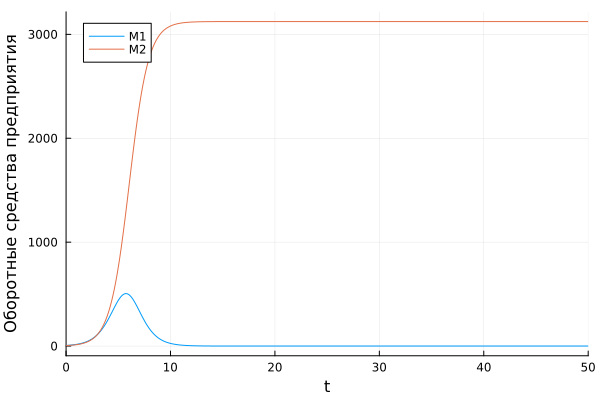
\includegraphics[width=0.7\textwidth,height=\textheight]{image/case2a.png}

}

\caption{\label{fig-008}График для случая 2}

\end{figure}%

\section{Реализация в
Scilab}\label{ux440ux435ux430ux43bux438ux437ux430ux446ux438ux44f-ux432-scilab}

Я создала такую же модель с помощью scilab

'\,'\,' p\_cr = 31; //критическая стоимость продукта tau1 = 15;
//длительность производственного цикла фирмы 1 p1 = 9.7; //себестоимость
продукта у фирмы 1 tau2 = 17; //длительность производственного цикла
фирмы 2 p2 = 8.4; //себестоимость продукта у фирмы 2 N = 30; //число
потребителей производимого продукта q = 1; //максимальная потребность
одного человека в продукте в единицу времени

a1 = p\_cr/(tau1\emph{tau1}p1\emph{p1}N\emph{q); a2 =
p\_cr/(tau2}tau2\emph{p2}p2\emph{N}q); b =
p\_cr/(tau1\emph{tau1}tau2\emph{tau2}p1\emph{p1}p2\emph{p2}N\emph{q); c1
= (p\_cr-p1)/(tau1}p1); c2 = (p\_cr-p2)/(tau2*p2);

// Случай 1 function dx=sysf(t, x) dx(1) = (c1/c1)\emph{x(1) -
(a1/c1)}x(1)\emph{x(1) - (b/c1)}x(1)\emph{x(2); dx(2) = (c2/c1)}x(2) -
(a2/c1)\emph{x(2)}x(2) - (b/c1)\emph{x(1)}x(2); endfunction

t0 = 0; x0 = {[}6.1; 4.5{]}; t = {[}0:0.01:50{]}; y = ode(x0, t0, t,
sysf); scf(1); plot(t, y); xlabel(\enquote{theta});
ylabel(\enquote{Оборотные средства предприятия}); legend({[}\enquote{M1}
\enquote{M2}{]}); xs2png(1, \enquote{case1.png});

// Случай 2 function dx=sysf2(t, x) dx(1) = (c1/c1)\emph{x(1) -
(a1/c1)}x(1)\emph{x(1) - (b/c1+0.00064)}x(1)\emph{x(2); dx(2) =
(c2/c1)}x(2) - (a2/c1)\emph{x(2)}x(2) - (b/c1)\emph{x(1)}x(2);
endfunction

y2 = ode(x0, t0, t, sysf2); scf(2); plot(t, y2);
xlabel(\enquote{theta}); ylabel(\enquote{Оборотные средства
предприятия}); legend({[}\enquote{M1} \enquote{M2}{]}); xs2png(2,
\enquote{case2a.png});

// Приближенный график для второго случая scf(3); plot(t, y2);
xlabel(\enquote{theta}); ylabel(\enquote{Оборотные средства
предприятия}); legend({[}\enquote{M1} \enquote{M2}{]});
zoom\_rect({[}0,0,50,2{]}); xs2png(3, \enquote{case2b.png}); '\,'\,' Я
получила те же графики, что и при использовании Julia(рис.9 и 10)

\begin{figure}

\centering{


\includegraphics[width=0.7\textwidth,height=\textheight]{image/pic2.png}

}

\caption{\label{fig-009}График для случая 1}

\end{figure}%

\begin{figure}

\centering{


\includegraphics[width=0.7\textwidth,height=\textheight]{image/pic3.png}

}

\caption{\label{fig-010}График для случая 2}

\end{figure}%

\chapter{Выводы}\label{ux432ux44bux432ux43eux434ux44b}

Делая эту лабораторную работу, я построила математическую модель
конкуренции двух фирм.

\chapter{Список
литературы}\label{ux441ux43fux438ux441ux43eux43a-ux43bux438ux442ux435ux440ux430ux442ux443ux440ux44b}

\begin{enumerate}
\def\labelenumi{\arabic{enumi}.}
\item
  Малыхин В.И. Математическое моделирование экономики. М., УРАО,
  1998.160 с.
\item
  Кулябов Д.С. Лабораторная работа 8. Модель конкуренции двух фирм
  {[}Электронный ресурс{]}
\end{enumerate}


\printbibliography


\end{document}
